\section{Theoretical Analysis}
\label{sec:analysis}

In this section we analyse the architecture chosen for the ACDC converter circuit using an Octave theoretical model. Using the ideal diode model we were able to predict the output of the Envelope Detector and Voltage Regulator circuits.

\subsection{Envelope Detector}

\begin{table}[h]
  \centering
  \begin{tabular}{|l|r|}
    \hline    
    {\bf Name} & {\bf Value} \\ \hline
    \input{initialdata_tab} 
  \end{tabular}
  \caption{Initial values for the input voltage and circuit components.}
  \label{tab:equivalent}
\end{table}
\subsection{Natural solution}
The natural solution for a node voltage dosen't take into account the independent sources of the circuit. The general solution for the natural regime in RC circuits, making use of the computations in the previous section, yields:
\begin{equation}
V_{6n}(t)=V_{6n}(\infty) + (V_{6n}(0) - V_{6n}(\infty))e^{(-\frac{t}{\tau})};
\end{equation}
The initial voltage in node 6 was obtained in the previous subsection, when we determined the equivalent resistor and the characteristic time. Calculating the $V_{6}$ node voltage in natural regime for t=$\infty$ is very simple - we need only to consider the same linear system of equations we used for our t$<$0 analysis, but this time $V_{s}$ = 0. Without any independent source powering the circuit, it is obvious that after an infinite amount of time the nodal voltages and branch currents will all be null. Nevertheless, we solved the system and our predictions checked out, as we can see in Table~\ref{tab:nule}.

From this equation, we computed the natural response in node 6, in the [0,20] milisseconds interval of time (Figure~\ref{fig:current}).

\begin{table}[h]
  \centering
  \begin{tabular}{|l|r|}
    \hline    
    {\bf Name} & {\bf Value [V]} \\ \hline
    \input{data_nule_tab} 
  \end{tabular}
  \caption{Node voltages for t=$\infty$.}
  \label{tab:nule}
\end{table}

\begin{figure}[h] \centering
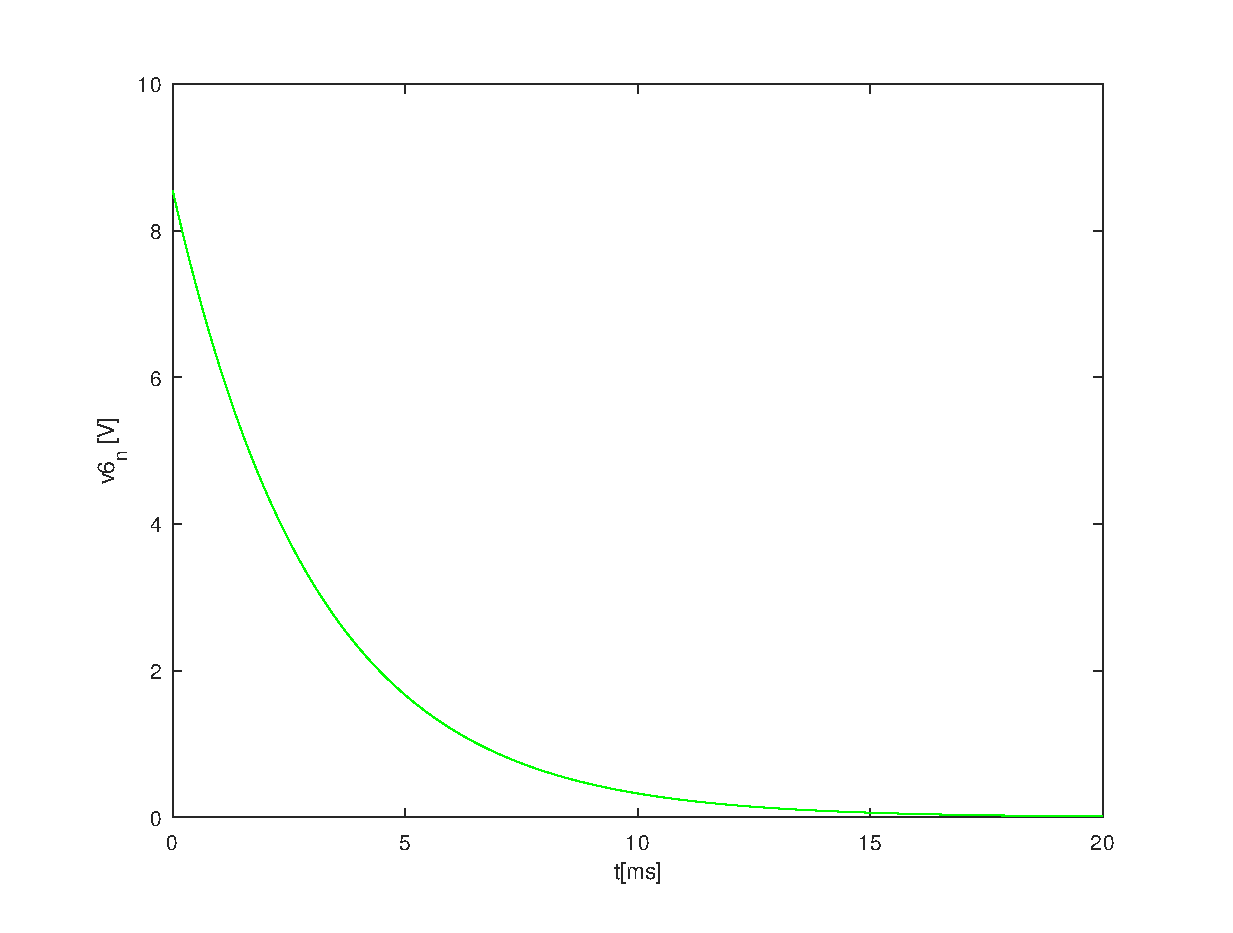
\includegraphics[width=0.7\linewidth]{natural.eps}
\caption{Natural solution to $V_{6}$ node voltage.}
\label{fig:current}
\end{figure}

\subsection{Forced solution}
In order to study the forced response of the system, we perform a nodal analysis to obtain the phasor voltage in every node. The voltage in every node will now be a function of the following type: $V = |V|e^{j(wt+\phi)}$, with the phasor expression given by $\tilde{V} = |V|e^{j\phi}$. Since there is only a single independent source acting in the circuit, every node voltage will oscillate with the same frequency - the source frequency - so we don't need to take frequency into acount in our nodal analysis and we can work solely on phasors. 

In this forced regime, the independent voltage source has a sinusoidal signal, with the following expression, $sin(wt)$, with $w=2\pi*f$ (in this study, we consider $f = 1kHz$). To perform the nodal analysis and determine the phasors' magnitudes and phases we must now work with impedances, instead of resistances and capacitance - the impedance of a resistor is $R$ and the impedance of a capacitor is given by $(\frac{1}{jwC})$. 

With all these definitions, we can now solve our linear system of equations:
\begin{equation}
\begin{pmatrix}
1 & 0 & 0 & 0 & 0 & 0 & 0\\
-G1 & G1+G2+G3 & -G2 & -G3 & 0 & 0 & 0\\
0 & Kb+G2 & -G2 & -Kb & 0 & 0 & 0\\
-G1 & G1 & 0 & G4 & 0 & G6 & 0\\
0 & 0 & 0 & 0 & 0 & -G6-G7 & G7\\
0 & 0 & 0 & 1 & 0 & G6*Kd & -1\\
0 & -G3 & 0 & G3+G4+G5 & -G5-jwC & G6 & jwC
\end{pmatrix}
\begin{pmatrix}
\tilde{V1}\\
\tilde{V2}\\
\tilde{V3}\\
\tilde{V5}\\
\tilde{V6}\\
\tilde{V7}\\
\tilde{V8}
\end{pmatrix}
=
\begin{pmatrix}
-j\\
0\\
0\\
0\\
0\\
0\\
0
\end{pmatrix}
\end{equation}
We then get these values:
\begin{table}[h]
  \centering
  \begin{tabular}{|l|r|r|}
    \hline    
    {\bf Name} & {\bf Amplitude [V]} & {\bf Phase [Degrees]}\\ \hline
    \input{eq2_tab} 
  \end{tabular}
  \caption{Phasor voltage for forced regime in every node.}
  \label{tab:phasor}
\end{table} \par
We're now able to make sense of the equation that describes the forced solution to the voltage at node 6.
\begin{equation}
V_{6f}(t)=V_{6r}cos(wt+V_{6\phi})=0.574648cos(2000\pi*t+1.7223);
\end{equation}
\subsection{Final total solution}
Now we convert the phasors to real time functions and consider an angular frequency of $2000\pi$. By superimposing both natural and forced responses we get the total solution:
\begin{equation}
V_{6}(t)=V_{6f}(t)+V_{6n}(t);
\end{equation}
By plotting both $V_s(t)$ and $V_6(t)$ from -5ms to 20ms we can see that both plots are constant before t=0 (Figure ~\ref{fig:tt}). The evolution of V6 is as expected, as we can clearly see the negative exponential behaviour as well as the induced frequency.
\begin{figure}[h] \centering
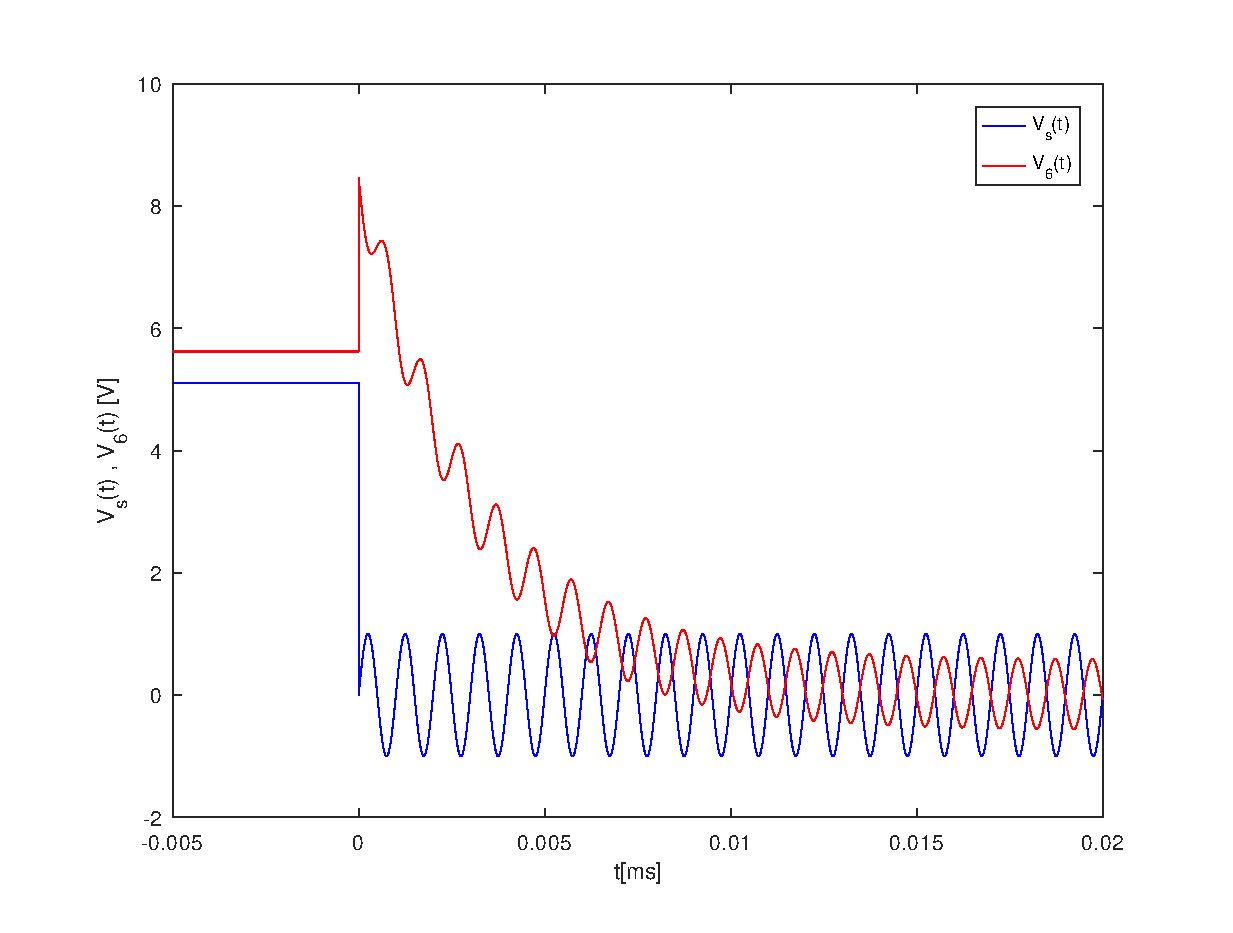
\includegraphics[width=0.7\linewidth]{total.eps}
\caption{Total solution to $V_{6}$ node voltage, compared to $V_{s}$ voltage source.}
\label{fig:tt}
\end{figure}
\subsection{Frequency response}
As we can see in the following plots, for low frequencies ($<$1Hz) every voltage is in phase. The capacitor is given enough time to charge up (asymptotically) to the same voltage as the voltage source, whose phase and magnitude remain constant throughout the analysed period. This means that at 0.1 Hz (period of 10 seconds), the capacitor charges and discharges in a fraction of a second and behaves like an open circuit for the rest of the cycle. We start seeing divergences in the graphs around the "cut-off frequency", defined as $\frac{1}{2\pi\tau}$, as we will see, which in our case is around 52Hz, explaining the changes happening between 10 and 10²Hz. When we consider a time interval in the same order of magnitude of $\tau$, the time it takes for a capacitor to deplete 36.8\% of its charge through a resistance, we are no longer giving the capacitor enough time to charge or discharge (almost) all the way. For much higher frequencies than the cut off, the capacitor starts behaving like a short circuit since it can no longer oppose the change of current (its reactance drops).
\begin{figure}[!h] 
	\centering
\begin{minipage}[b]{0.65\linewidth}	
	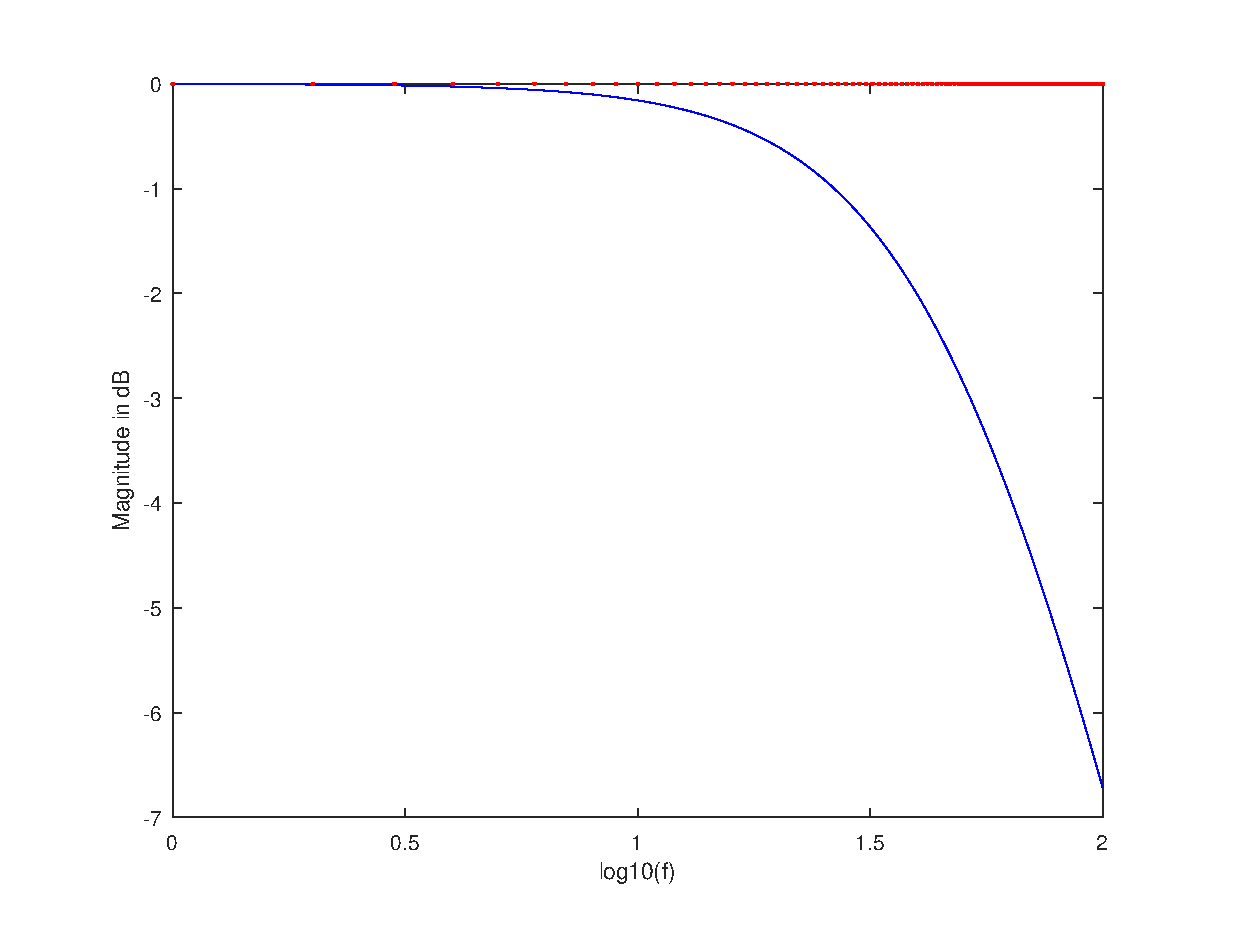
\includegraphics[width=\linewidth]{magnitude.eps}
\caption{Variation with frequency of $V_{s}$, $V_{6}$ and $V_{c}$ voltage magnitudes (in dB).}
\end{minipage}
\hfill
\begin{minipage}[b]{0.65\linewidth}
\includegraphics[width=\linewidth]{phase.eps}
\caption{Variation with frequency of $V_{s}$, $V_{6}$ and $V_{c}$ voltage phases.}
\end{minipage}
\end{figure}
The apparent phase discontinuity is only due to the use of the arctan function, whose output is bounded by [-180,180] until it circles back around to the top. So the phase is in fact continuous.
The following equations help describe the behaviour shown in the plots. They come from reducing the circuit to a sinusoidal voltage source, equivalent resistance and a capacitor.
\begin{equation}
\tilde{V_c}=\frac{\tilde{V_i}}{1+j(R_{eq}C)2\pi*f}
\end{equation}
\begin{equation}
|\tilde{V_c}|=\frac{|\tilde{V_i}|}{\sqrt{1+((R_{eq}C)2\pi*f)^2}}
\end{equation}
\begin{equation}
\phi V_c=-\frac{\pi}{2}-arctan((R_{eq})C2\pi*f)
\end{equation}

Converting the magnitude equation to dB, we encounter a term from which the "cut-off" angular frequency appears, equal to $\frac{1}{R_{eq}C}$ : $-10\log_{10}(1+w^2(R_{eq}C)^2)$. In an other form, the "cut-off" frequency can be defined as the point of intersection of two asymptotes: the horizontal asymptote for frequencies close to zero and the oblique asymptote, for very high frequencies. Once again, after this point the voltage stored in the capacitor starts dropping considerably.

In the magnitude plot of the $V_{6}$ node voltage, we have two horizontal asymptotes, one for frequencies very close to zero, other for very high frequencies, which means the node voltage remains constant for low frequencies, transforming then when the "cut-off" frequency is achieved, stabilizing afterwards at a lower value for very high frequencies. The same process happens regarding the $V_{6}$ phase: at an early stage the phase is of course the source's -90 degrees, but then transforms stabilizing at an opposite phase of 90 degrees. The $V_{c}$ phase variation is well described in Equation 13, starting at the before mentioned -90 degrees, and settling at a -180 degrees phase - for very high frequencies, the $V_{c}$ and $V_{6}$ voltages are not in phase anymore - with such a high frequency, $V_{8}$ is not given enough time to phase-in in relation to $V_{6}$.

